\section{Model trained on the merged data}
% obidva modeli ze dame testovat
% tabulka s vysledkami na provonanie
% vyjadrenie ze ktory je lepsi
% ukazat matice a acc, recall ... 
% tuto asi bude dobre spravit subsubsection a tam kazdy model opisat
% a potom spravit dalsiu kde ich porovnam nejak

% este to porovnat aj s resnetom nejak

On the testing dataset, the model from Section \ref{subsec:mergedmodel} has achieved an accuracy of 87.00 \%, precision of 87.15 \% and recall of 87.00 \%. Of 300 images only 39 were wrongly classified. 

From the confusion matrix in the Figure \ref{img:confmatrixmerged} we can see that the model has classified 14 cases of galaxies as streaks. This could be caused again by the fact that several samples of galaxies have a sharp elliptical shape that resembles a streak (\ref{fig:galaxystreakmis2}). 
Apart from this only a small amount of misclassified images is with streak and galaxy (5 cases), streak and point (4 cases) and cosmic rays and hot pixels (4 cases). Some cases of the wrongly classified images are depicted in the Figure \ref{fig:wrongmerged}. We can see that a cosmic ray which has very few pixels have been classified as a hot pixel (\ref{fig:cosmichotpixelmis}), or a very short streak was predicted as a point (\ref{fig:streakpointmis2}). 

\begin{figure}[h]
    \centering
    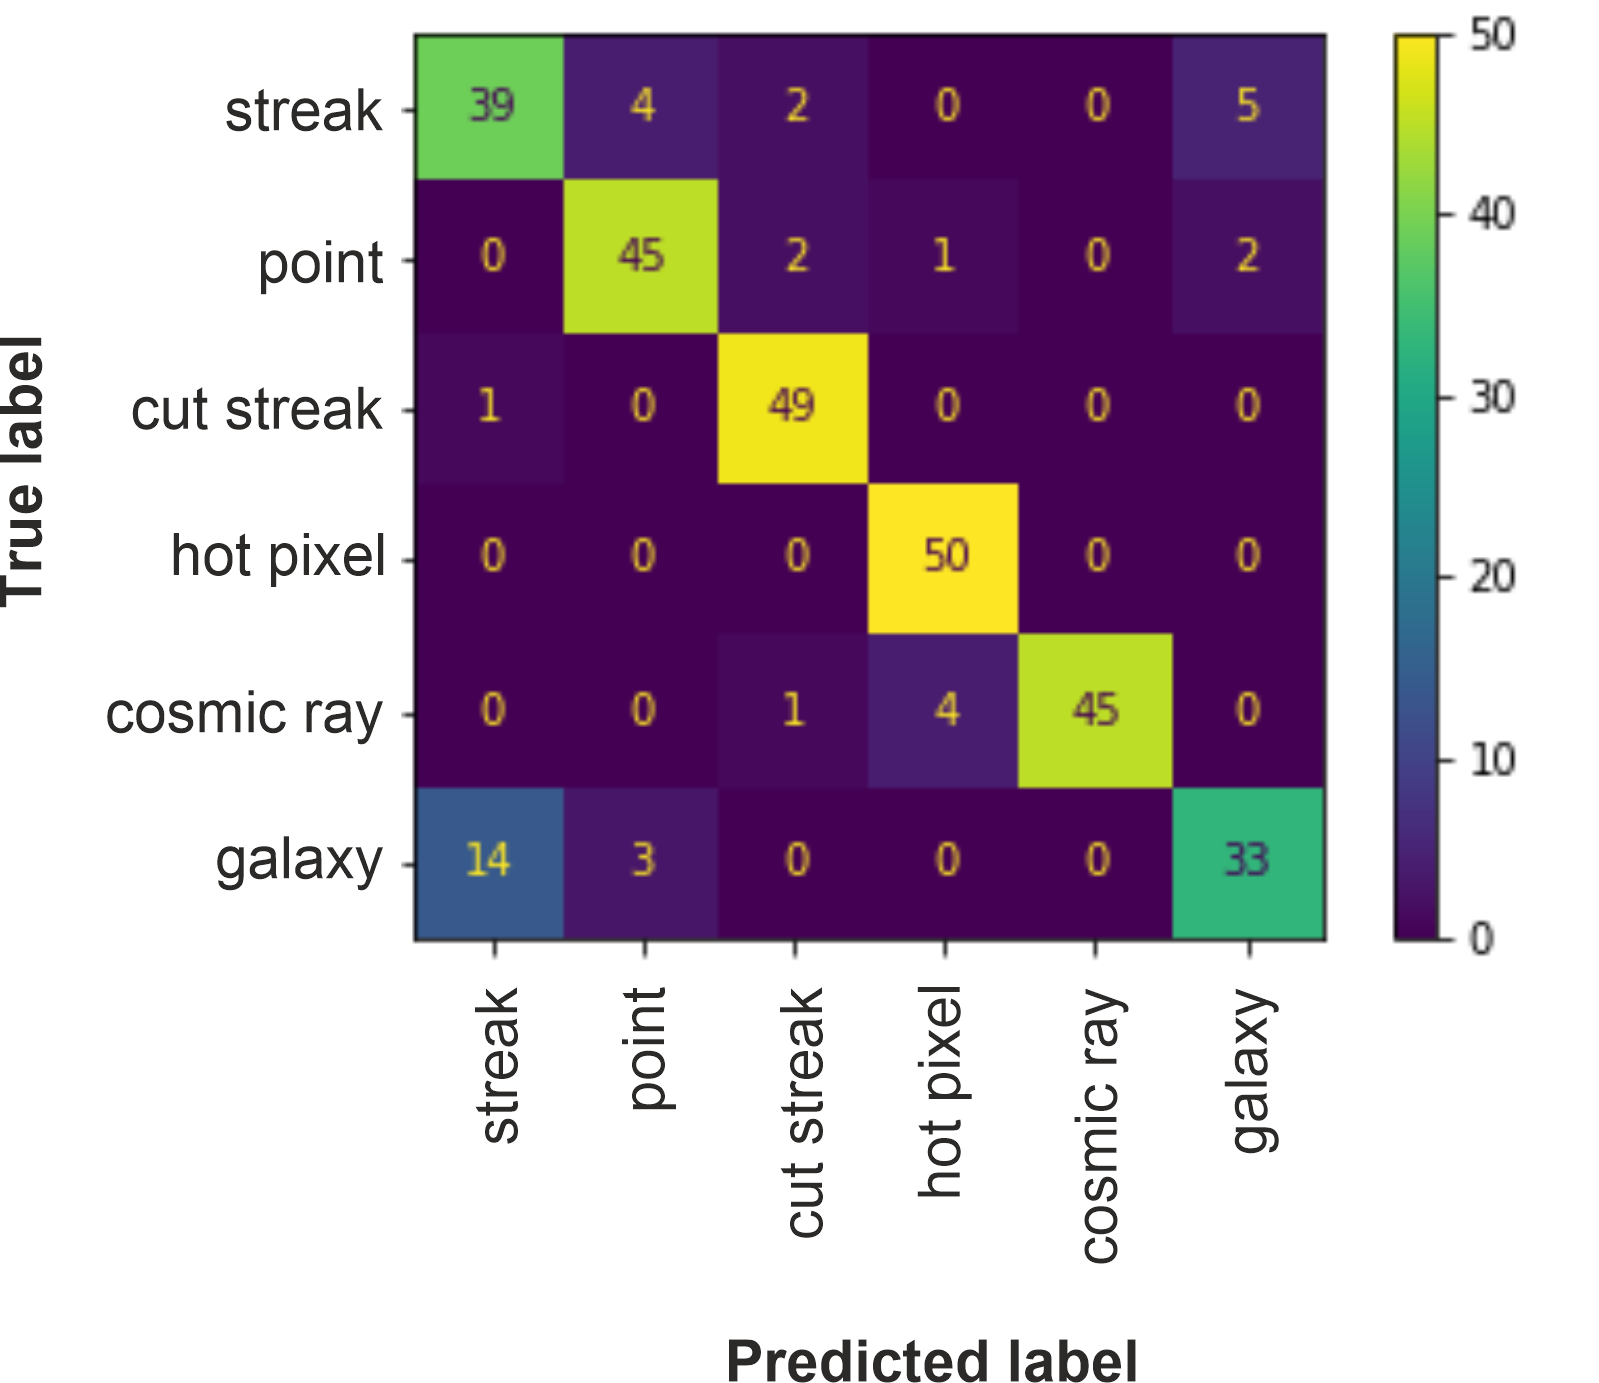
\includegraphics[width=.5\textwidth]{images/confusionMatrix13r_0.png}
    \caption{Confusion matrix from the testing of the model trained on merged synthetic and real data.}
    \label{img:confmatrixmerged}
\end{figure}

\begin{figure}[!h]
\centering
    \begin{subfigure}[t]{.23\textwidth}
        \centering
        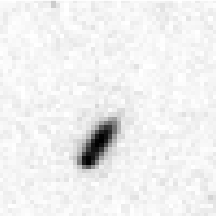
\includegraphics[width=\textwidth]{images/mwrongImage10.png}
        \caption{}
        \label{fig:galaxystreakmis2}
    \end{subfigure}
    \begin{subfigure}[t]{.23\textwidth}
        \centering
        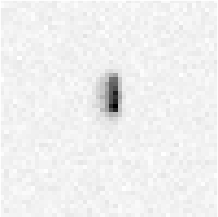
\includegraphics[width=\textwidth]{images/mwrongImage2.png}
        \caption{}
    \end{subfigure}
    \begin{subfigure}[t]{.23\textwidth}
        \centering
        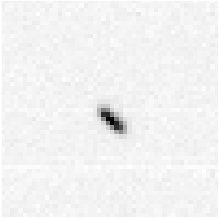
\includegraphics[width=\textwidth]{images/mwrongImage26.png}
        \caption{}
        \label{fig:streakpointmis2}
    \end{subfigure}
    \begin{subfigure}[t]{.23\textwidth}
        \centering
        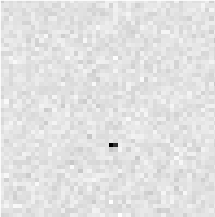
\includegraphics[width=\textwidth]{images/mwrongImage28.png}
        \caption{}
        \label{fig:cosmichotpixelmis}
    \end{subfigure}

    \caption[Wrongly classified images on the model that trained with merged synthetic and real data. ]
    {Wrongly classified images on the model that trained with merged synthetic and real data. (a) A galaxy misclassified as a streak, (b) A streak misclassified as a galaxy, (c) A streak misclassified as a point, (d) A cosmic ray misclassified as a hot pixel. }
    \label{fig:wrongmerged}
\end{figure}
